%%%%%%%%%%%%%%%%%%%%% chapter.tex %%%%%%%%%%%%%%%%%%%%%%%%%%%%%%%%%
%
% sample chapter
%
% Use this file as a template for your own input.
%
%%%%%%%%%%%%%%%%%%%%%%%% Springer-Verlag %%%%%%%%%%%%%%%%%%%%%%%%%%

\chapstarthook{El contenido del cap�tulo corresponde con el art�culo: \textbf{J.A. Aguilar, I. Garrig{\'o}s, J.-N. Maz{\'o}n, J. Trujillo. An MDA Approach for Goal-oriented Requirement Analysis in Web Engineering. Journal of Universal Computer Science (J.UCS), 16(17): 2475-2494 (2010).}}


\chapter{An MDA Approach for Goal-oriented Requirement Analysis in Web Engineering}
\label{c4} % Always give a unique label
% use \chaptermark{}
% to alter or adjust the chapter heading in the running head

%Since the previous chapter has defined how to obtain a
%relational-based implementation of the multidimensional conceptual
%model, this chapter focuses on obtaining a logical representation
%directly based on multidimensional technology, thus showing the full
%potential of applying formal transformations within a model-driven
%approach. The content of this chapter corresponds with the part of
%the approach shaded in the figure below.

\begin{figure}[h!]
  \begin{center}
    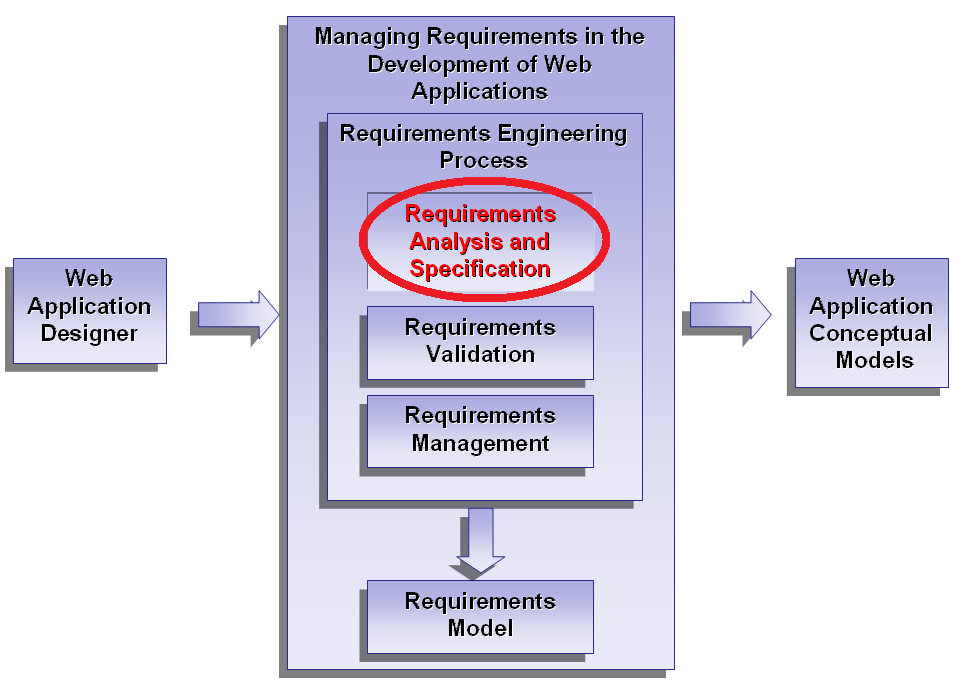
\includegraphics[width=0.7\textwidth]{img/PropuestaCap1.png}
  \end{center}
  %\caption{} \label{}
\end{figure}

Se presenta el Cap�tulo \ref{c4}, a raz�n de que los resultados obtenidos en el Cap�tulo \ref{c3} muestran, entre otras cosas, que gran parte de las metodolog�as Web no ofrecen un soporte integral en la etapa de an�lisis y especificaci�n de requisitos.

El Cap�tulo \ref{c4} describe una metodolog�a para la gesti�n de requisitos en ingenier�a Web. La metodolog�a est� basada en el marco de modelado orientado a objetivos \emph{i*} y en MDA (\emph{Model-Driven Architecture}). La propuesta le permite al dise�ador de la aplicaci�n Web derivar la estructura de los modelos conceptuales que conforman la aplicaci�n a partir de la especificaci�n de requisitos. 


%This chapter was published in the \emph{International Conference on
%Data Warehousing and Knowledge Discovery (DaWaK)}. This conference
%has become one of the most important international scientific events
%through which to bring together researchers, developers and
%practitioners to discuss the latest research issues and experiences
%in developing and deploying data warehousing and knowledge discovery
%systems, applications, and solutions. Each year, \emph{DaWaK} seeks
%to introduce innovative principles, methods, algorithms and
%solutions to challenging problems faced in the development of data
%warehousing, knowledge discovery and data mining applications.
%\emph{DaWaK} is, therefore, a leading international forum for the
%presentation and discussion of current research and applications in
%which the major emphasis is on data warehousing. The high quality of
%this conference can be demonstrated through the following two facts:
%the \emph{acceptance rate} of this conference is usually around
%\emph{30\%}, and the \emph{Estimated Impact of Conference (EIC)} is
%\emph{0.86} according to \emph{The Computer Science Conference
%Ranking Website}
%(\url{http://www.cs-conference-ranking.org/home.html}).


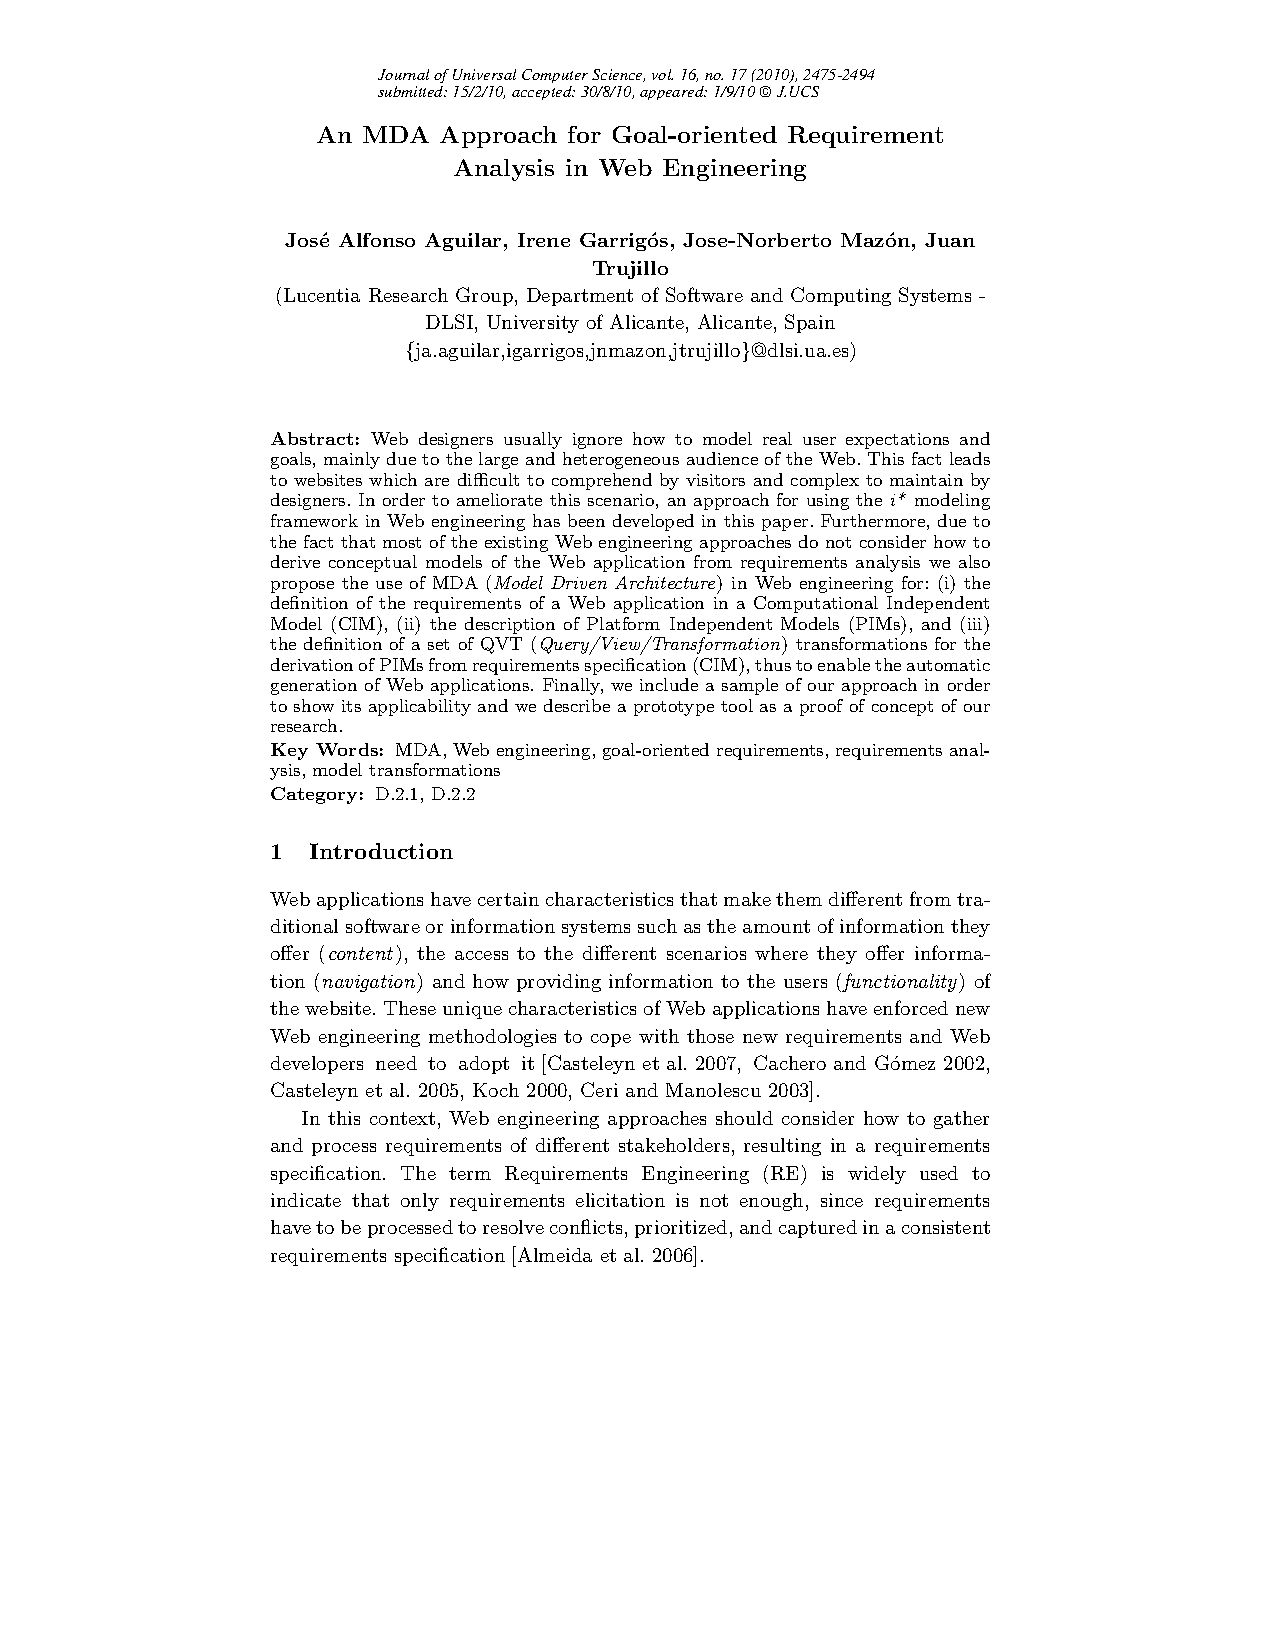
\includepdf[openright=true,pages={1-20}]{papers/JUCS2010.pdf}
%
